\chapter{Sound Source Localization \& \library{Mirage}}\label{chap:mirage}

\marginpar{%
    \footnotesize
    \textbf{Keywords:} Sound Source Localization, Image Microphones, Acoustic Echoes, TDOA Estimation.
    \\\textbf{Resources:}
    \begin{itemize}
        \item \href{https://ieeexplore.ieee.org/document/8683534}{Paper}
        \item \href{https://github.com/Chutlhu/mirage}{Code}
        \item \href{https://sigport.org/documents/mirage-2d-sound-source-localization-using-microphone-pair-augmentation-echoes}{Poster}
        \item \href{https://www.youtube.com/watch?v=SfEmwqxxpYg}{Haru Robot presentation}
    \end{itemize}
}

\newthought{Synopsis} \synopsisChMirage

\mynewline
Together with~\cref{ch:lantern}, this chapter describes methods and results published in~\cite{di2019mirage}, which considers only stereophonic recordings.
In this sense, this chapter provides an application of the~\cref{ch:lantern}.
Subsequently, the proposed approach was to multi-microphone recordings in collaboration with Randy Gomez from Honda Research Institute.
\marginpar{
    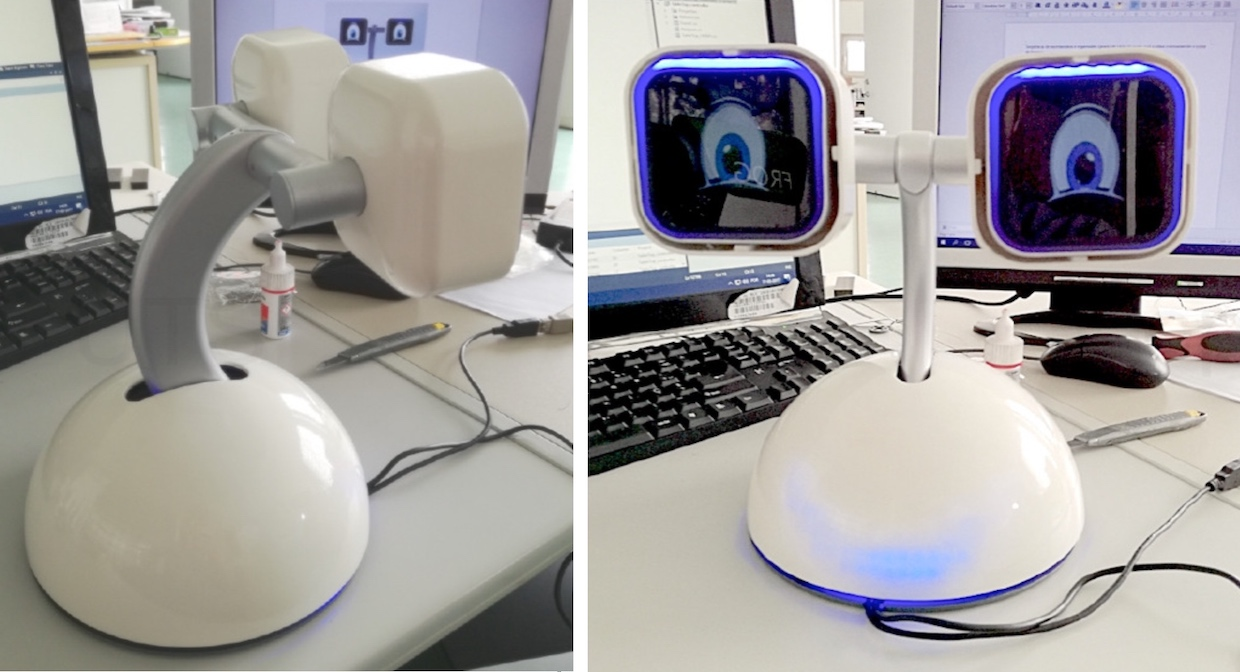
\includegraphics[width=\linewidth]{mirage/haru.jpeg}
    \captionof{figure}{The Haru Robot}
    \label{fig:mirage:haru}
}
In particular, the method was tested on an autonomous robot platform called \library{Haru}\citeonly{ackerman2018haru, gomez2018haru}, consisting of a base and two screens mimicking a face with two eyes (See~\cref{fig:mirage:haru})
The robot will be fitted with actuators (for the whole body, the neck, and the eyes) and cameras and a microphones for visual and auditory sensing.
The partner agreed on using its technology to see the impact of echo-aware sound source localization.
Therefore, the multichannel extention of this method consider the circular microphone array featuring 7 sensor of the \library{Haru} robot.
The results of this study was described in an internal technical report~\cite{di2019honda}.


\section{Literature review in Echo-aware Sound Source Localization}
Common to most sound source localization approaches reviewed in ~\cref{subsec:application:localization} is the challenge posed by environment reverberation.
It is typical to observe that \ac{DOAs} estimation degrades with increasing acoustic reflection~\citeonly{chen2006time}.
For these reasons, most sound source localization methods regard reverberation and, in particular, acoustic echoes as a nuisance.
Room reverberation is considered in the works~\citeonly{rui2004time, chen2006time, zhang2007maximum} while the authors of~\citeonly{weinstein1994iterative, taghizadeh2015spatial, salvati2016sound} attempt to solve \SSL/ by estimating the full \RIRs/.
However, both the cases have drawbacks: in the former, the generic model for reverberation does not reduce strong early echoes, and in the latter, \RIRs/ estimation is a difficult task.

\mynewline
The echo-aware sound source localization methods take another direction: they exploit the closed-form relation between echoes timings and audio scene geometry expressed by the \ISMdef/.
Early works such as~\citeonly{korhonen2008acoustic, ribeiro2010turning, ribeiro2010using, svaizer2011use} uses knowledge form the room geometry to estimated the position of the sound source with respect to the arrays.
This idea was subsequently extended in later works, reducing the amount of prior knowledge required or addressing different applications.
The authors of \citeonly{nakashima2010localization}  study the \SSL/ problem in binaural recordings.
To improve localization, they propose to used ad-hoc reflectors as artificial \textit{pinnae} and a simple reflection model.
In the work~\citeonly{krekovic2016echoslam}, the author addresses the problem \ac{SLAM}\sidenote{
    \ac{SLAM} enables the estimation of a moving robot’s position in relation to a number of external acoustic sources.
} using echoes.
The authors of~\citeonly{an2018reflection} propose to use cameras, depth sensors, and laser sensors to identify reflectors and build a corresponding acoustic model that is used
for echo-aware \ac{SSL}.
Finally, in a very recent work, the well-known \ac{MUSIC} framework for localizing multiple sources is modified for accounting an echo model for the spherical harmonic representation~\citeonly{birnie2020reflection}

\mynewline
All the above mentioned echo-aware methods are explicitly knowledge-driven, namely, using closed-form solutions based on physics, acoustics, and signal processing models.
As explained in the previous chapter, data-driven methods, especially \ac{DNN}, have been successfully applied to address \SSL/.
The main benefit is in their ability to learn complex mapping functions based on simple input-output pairs.
However, they are typically trained for specific applications and use-cases (\eg/, arrays geometry, acoustic conditions, \etc/) and fail whenever test conditions strongly mismatch training conditions.

\section{Proposed Approach}
In the work \cite{di2019mirage}, we proposed to combine the best of the two worlds:
using a deep learning model to estimate challenging acoustic parameters and a physically-motivated model to map such parameters to source's \DOAs/.
To this end, we introduce the framework of \MIRAGEdef/ for \SSL/, based on the \textit{image microphones} model~\citeonly{bergamo2004collaborative,korhonen2008acoustic} (See~\cref{sec:separake:sota}).

\mynewline
Let us consider a simple yet common scenario to illustrate this idea:
two microphones, one source, and a nearby reflective surface, as illustrated in Fig. \cref{fig:mirage:scene}.
\marginpar{%
    \centering
    \footnotesize
    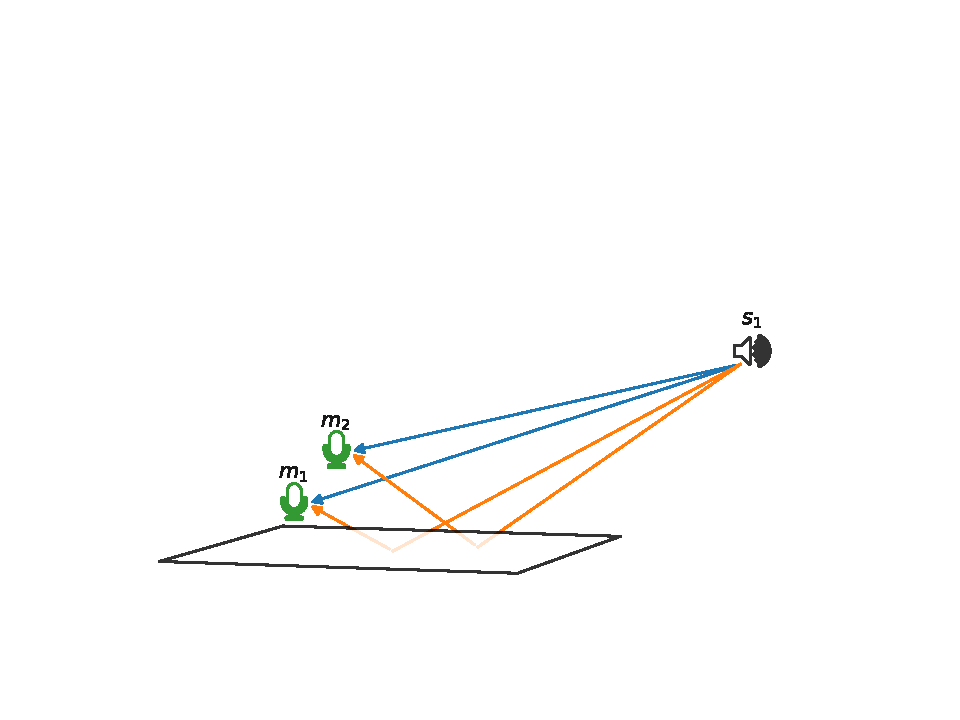
\includegraphics[trim={50 70 50 150},clip,width=\linewidth]{mirage/scene.pdf}
    \captionof{figure}{%
        Typical setup with one source source recorded by two microphones.
        The illustration shows direct sound path (blue lines) and resulting first-order echoes (orange lines).}
    \label{fig:mirage:scene}
}
This may occur when the sensors are placed on a table or next to a wall. Striking examples of these scenarios are the smart table-top devices, such as Amazon Echo, Google Home, \etc/.
The reflective surface is assumed to be the most reflective and closest one to the microphones in the environment, generating the strongest and earliest echo in each microphone.
Under this \textit{close-surface} model, we ask the following question:
\begin{enumerate}
    \item Can early echoes be estimated from two-microphone recordings of an unknown source?
    \item Can early echoes be used to estimate both the azimuth and elevation angles of the source, an \textit{impossible} task in free field conditions?
\end{enumerate}

\newthought{The First Question} was already addressed in~\Cref{ch:lantern}.
In particular, we proposed to use a \ac{DNN} trained on a simulated close-surface dataset to estimate early echoes properties from audio features.

\newthought{To answer the Second Question}, we propose the \ac{MIRAGE} framework.
It exploits echoes' time of arrival by expressing them as \acp{TDOA} in the \textit{virtual 4-microphone array} formed by the true microphone pair and its image with respect to the reflective surface.
We show that this framework approximately estimates echo properties, perform similarly to a correlation-based method in azimuth estimation for the considered
scenario and estimates \textit{impossible} elevation angles with good accuracy in noiseless settings using two microphones only.



\section{Background in microphone array SSL}\label{sec:background}
In this section, we briefly review some necessary background in microphone array \ac{SSL}.
Let us assume a microphone array of $\idxMic$ sensors is placed inside a room and records the sound emitted by one static point sound source ($\numSrcs=1$).
In all generality, the relationship between the signal $\mic_\idxMic$ recorded by the $\idxMic$-th sensor placed at fixed position $\positionMicrophone_\idxMic$ and the signal $\src$ emitted by the source at fixed position $\positionSource$ is defined by:
\begin{equation}\label{eq:mirage:anymic_time}
\mic_i[n] = (\flt_\idxMic \convDis \src)[n]  \; + \; \nse_\idxMic[n],
\end{equation}
where the convolution with \RIR/ $\flt_\idxMic[n]$ embodies the fact that sensor $\idxMic$ receives a spatial image of the source and $\nse_\idxMic$ denotes possible measurement noise.
As fully described in~\cref{ch:acoustic}, the \RIR/ depends on the spatial parameters of the scene: microphone positions, source position \wrt/ the room, as well as the room acoustic properties (size, absorption, and diffuseness of the wall materials).

\mynewline
Let us assume that \RIRs/ follows the echo model under the narrowband approximation presented in~\cref{subsec:processing:stft}.
Therefore, in the discrete-frequency domain, this leads to
\begin{equation}\label{eq:mirage:rir}
    \FLT_\idxMic[k] = \sum_{\idxEch=0}^{\numEchs}  \; \alpha_\idxMic^{(\idxEch)}[k] \; \cste^{- \csti 2 \pi f_k \tau_\idxMic^{(\idxEch)}} \; + \; \varepsilon_\idxMic[k],
\end{equation}
where $f_k$ is the $k$-th frequency bin and the error term $\varepsilon_i[k]$ collects later echoes, the reverberation tail, diffusion, and noise.
In this work, we will consider only the first strongest echo, therefore $R = 1$.
Note that for $r=0$ denotes the ideal propagation path,
being $\tau^{(0)_\idxMic}$ the ideal propagation path from the source to the $\idxMic$-th microphone, and $\alpha^{(0)_\idxMic}$ the air attenuation.
In the remainder of this work, we make the approximation of $\alpha_i^{(\idxEch)}$ being frequency-independent.

\subsection{2-channel 1D-SSL}\label{subsec:mirage:1D-SSL}
\newcommand{\tdoa}{\ensuremath{\tau_\mathtt{TDOA}}}
\newcommand{\aoa}{\ensuremath{\vartheta}}
Let us first consider the case of stereophonic recordings ($\numMics=2$).
Under the far- and free-field assumption, traditional \SSL/ methods use the \acf{TDOA},
\begin{equation*}
    \tdoa \eqdef \tau^{(0)}_2 - \tau^{(0)}_1\quad\text{[second]}
    ,
\end{equation*}
as a proxy for the estimation of the \ac{AOA}, $\aoa$, since:
\begin{equation}\label{eq:mirage:aoa}
    \vartheta = \arccos \kparen{\speedOfSound \: \tdoa \: / \: \distMicMic }\quad\text{[rad]},
\end{equation}
where $\speedOfSound$ is the speed of sound and $\distMicMic$ the inter-microphone distance.

\begin{figure}
    \begin{sidecaption}[]{
        Illustration of the relation between \ac{DOA} and \ac{TDOA} with ones source and two microphone.
        Knowing the distance $\distMicMic$ between the two microphones, simple trigonometry yields the \ac{AOA} $\vartheta$ according to~\cref{eq:mirage:aoa}.
    }[fig:mirage:gcc]
        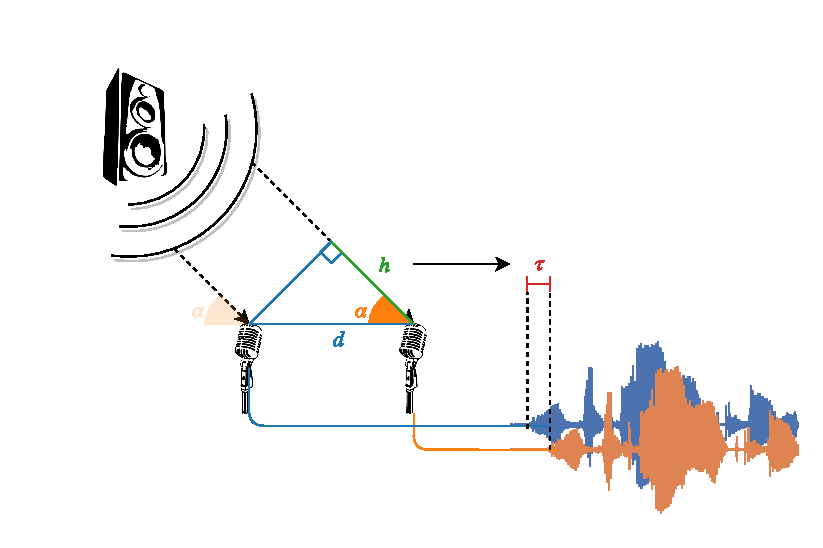
\includegraphics[width=\linewidth]{mirage/tdoa_microphone.pdf}
    \end{sidecaption}
\end{figure}


\mynewline
Then, \SSL/ reduces to estimating the \ac{TDOA}, which can be done by \ac{CC}-based methods such as the widely used and well performing \ac{GCC-PHAT} method \citeonly{knapp1976generalized, blandin2012multi}.
Given \STFT/ $\MIC_1$ and $\MIC_2$ of the two microphones signals, the \ac{CC} and \ac{GCC-PHAT} \textit{angular spectra} are defined as:\marginpar{
    \footnotesize\itshape
    The ``generalized'' cross-correlation methods adds weighting functions (\eg/ the phase transfor (PHAT),  or the smoothed coherence transform (SCOT))
    to the \ac{CC}. Their purpose is to improve the estimation of the time delay on specific characteristic of the signal and noise.
    See~\citeonly{chen2006time} for an overview.
}
\begin{equation}\label{eq:mirage:cc}
    \Psi_\mathtt{CC}(\tau) = \sum_{k,l} \MIC_1[k,l] \khermitian{\MIC}_2[k,l] \cste^{-\csti 2  \pi f_k \tau}
    ,
    \end{equation}
\begin{equation}\label{eq:mirage:gccphat}
    \Psi_\mathtt{PHAT}(\tau) = \sum_{k,l}\frac{\MIC_1[k,l] \khermitian{\MIC}_2[k,l]}{\kvbar{ \MIC_1[k,l] \khermitian{\MIC}_2[k,l] }} \cste^{-\csti 2  \pi f_k \tau}
    ,
\end{equation}
where $\kvbar{\cdot}$ denotes the absolute value and the weighting function $1 / \kvbar{ \MIC_1[k,l] \khermitian{\MIC}_2[k,l]}$ is called \textit{phase transform},
aiming at reducing the source's autocorrelation component from the angular spectrum.

\mynewline
Then, the \ac{TDOA} estimate is given by
\begin{equation*}
    \hat{\tau}_\mathtt{TDOA} = \arg \underset{\tau}{\max} \; \Psi_\mathtt{PHAT}(\tau) \qquad [\text{\resp/}\; \Psi_\mathtt{CC}(\tau)]
    .
\end{equation*}
Note that $\Psi_\mathtt{PHAT}$ [\resp/ $\Psi_\mathtt{CC}$] can also be expressed directly as a function of the \ac{AOA} using \eqref{eq:mirage:aoa}, hence the term \textit{angular spectrum}.
Despite the theoretical limits of this method, discussed in~\citeonly{chen2006time}, this method is known to work well in practice.
Moreover, it was showed to be state-of-the-art for \ac{SSL} in a large benchmark study~\citeonly{blandin2012multi}.

\subsection{Multichannel 2D-SSL}\label{subsec:mirage:2D-SSL}
When more microphones are available and the microphones array is compact and not linear\sidenote{
    In case of complanarity, the angle can be estimated up to ``up-down'' umbigity.
}, 2D-\ac{SSL} can be envisioned
A possible approach is to use 1D-\ac{SSL} on all pairs and combine their results, a principle which was successfully applied in the \acf{SRP-PHAT} method \citeonly{dibiase2001robust}.


\mynewline
\begin{figure}
    \begin{sidecaption}[t]{
        Illustration of the different \acp{DOA} at each microphone pairs listening one sound source.
        Knowing the position of the microphone, the angle with respect to a reference point can be deduced in closed-form.
    }[fig:mirage:gcc]
        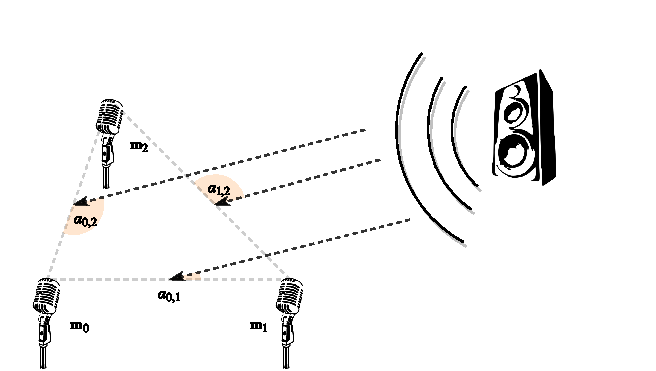
\includegraphics[width=\linewidth]{mirage/srp-phat_aggregation.pdf}
    \end{sidecaption}
\end{figure}
The \ac{SRP-PHAT} methods returns the source's \ac{DOA}, namely the pair azimuth and elevation $(\theta, \phi)$, by estimating \acp{TDOA} from each microphone pairs.
In order to achieve this, it requires the geometry of the microphone array to be known.
In a nutshell, this algorithm aims to estimate a \textit{global angular spectrum} $\Psi_{\mathtt{SRP}}(\theta,\phi)$ in the polar coordinates system with respect to reference point in the array, typically its barycenter.
This function will exhibit a local maximum in the direction of the active source.
\\The algorithmic can be exemplified in the following steps:\marginpar{
    \footnotesize\itshape
    See \href{http://bass-db.gforge.inria.fr/bss_locate/}{\library{MBSSLocate}\ExternalLink} for a free MATLAB implementation and comprehensive documentation of this algorithm.
}
\begin{enumerate}
    \item a global grid of \acp{DOA} candidates is defined according to a desired resolution and computational load;
    \item for each pair of microphones, a local set of \ac{AOA} (hence, \acp{TDOA}) is defined based on the above chosen \acp{DOA} and the input geometry;
    \item a TDOA-based algorithm (\eg/ \ac{GCC-PHAT}) is used to compute the associated local angular spectrum;
    \item all the local contributions (a collection of local $\Psi_\mathtt{GCC}(\tau)$) are geometrical aggregated and interpolated back to the global \ac{DOA} grid to form $\Psi_{\mathtt{SRP}}(\theta,\phi)$;
    \item the \acs{DOA}(s) maximizing $\Psi_\mathtt{SRP}$ is (are) used as estimate (in case of multiple sources).
\end{enumerate}
This algorithm can be seen as an application of the divide-and-conquer paradigm to \ac{TDOA}-based methods:
``at the leaves'', the \ac{GCC-PHAT} method provide \ac{TDOA} for each microphone pair;
the ``merge'' operation consists in aggregating \ac{TDOA} defined on a different axis based on the knowledge of the array geometry.
Finally, we stress that this algorithm is independent of the method used to estimate the \ac{TDOA}.

\section{MIRAGE: Microphone Array Augmentation with Echoes}\label{sec:mirage:mirage}
We now introduce the proposed concept of \MIRAGEdef/.
Eq.~\cref{eq:mirage:echo_h} then corresponds to the well known image-source (IS) model,
where reflections are treated as mirror images of the true source with respect to reflective surfaces,
emitting the same signal.
\marginpar{%
\centering
\footnotesize
    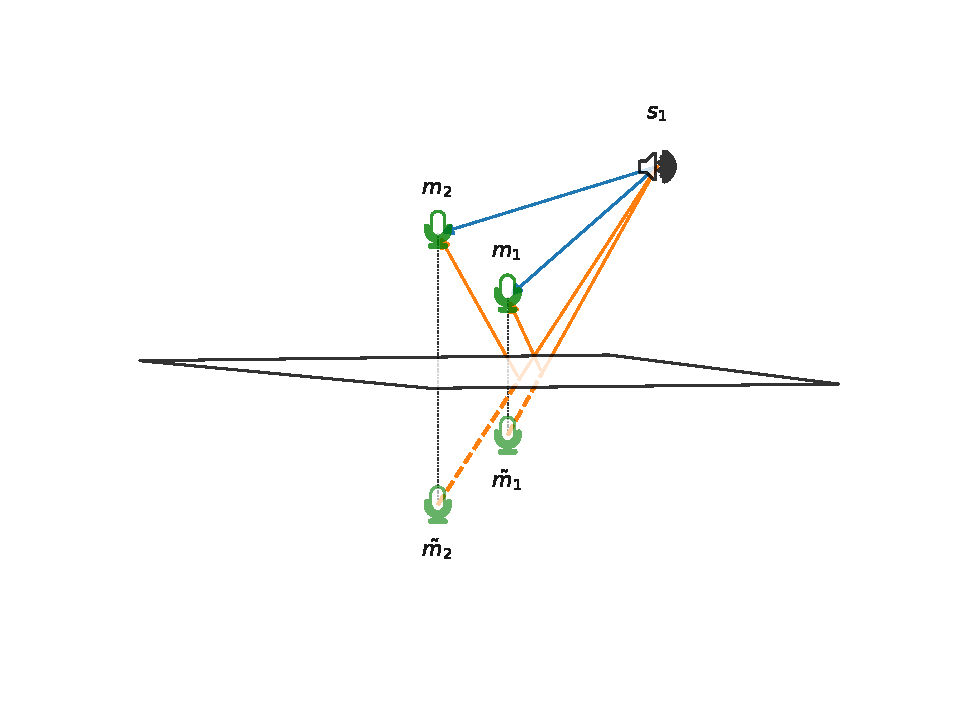
\includegraphics[trim={90 75 40 50},clip,width=\linewidth]{mirage/mirage.pdf}
    \captionof{figure}{%
        Illustration of the images $\mathring{\positionMicrophone}_1$ and $\mathring{\positionMicrophone}_2$ of microphones $\positionMicrophone_1$ and $\positionMicrophone_2$ in the presence of a reflective surface and a source.
        Blue lines correspond to direct paths, orange lines correspond to echo paths.}
    \label{fig:mirage:mirage}
}
We will employ here a less common but equivalent interpretation of IS,
namely, the image-microphone (IM) model. As illustrated in Fig.~\cref{fig:mirage:mirage},
virtual microphones are mirror images of the true microphones with respect to reflective surfaces.
In this view, the echoic signal received at a true microphone
is the sum of the anechoic signals received at this microphone and its images.
If we consider the virtual array consisting of both true and image microphones,
multiple microphone pairs are now available. For each of them,
it is then possible to define a corresponding time difference of arrival.
Among them, we will refer to the one between the two real microphones as \ac{TDOA}, the one between the two image microphones as \ac{iTDOA} and the one between the first microphone and its image as \ac{TDOE}.
Therefore, we have:
\begin{align}
\tau_\mathtt{TDOA}  &= \tfrac{1}{c} \norm{\positionMicrophone_2 - \positionSource} - \tfrac{1}{c} \norm{\positionMicrophone_1 - \positionSource} = \tau_2^{(0)} - \tau_1^{(0)},\\
\tau_\mathtt{iTDOA} &= \tfrac{1}{c} \norm{\mathring{\positionMicrophone}_2 - \positionSource} - \tfrac{1}{c} \norm{\mathring{\positionMicrophone}_1 - \positionSource} = \tau_2^{(1)} - \tau_1^{(1)},\\
\tau_{\mathtt{TDOE},1}  &= \tfrac{1}{c} \norm{\mathring{\positionMicrophone}_1 - \positionSource} - \tfrac{1}{c} \norm{\positionMicrophone_1 - \positionSource} = \tau_1^{(1)} - \tau_1^{(0)}\\
\end{align}
where $\mathring{\positionMicrophone}_i$ denotes the position of the image of $\positionMicrophone_i$ with respect to the reflector.
Note that $\tau_{\mathtt{TDOE},2} = \tau_\mathtt{iTDOA} + \tau_{\mathtt{TDOE}, 1} - \tau_\mathtt{TDOA}$.
These three quantities are directly connected to \RIRs/, as illustrated in Fig.~\cref{fig:mirage:rirs} (Right).
Let $V = \set{\tau_{\mathtt{TDOA}}, \tau_{\mathtt{iTDOA}}, \tau_{\mathtt{TDOE},1}}\in\mathbb{R}^3$


\begin{figure}[t]
    \begin{sidecaption}[RIRs within the MIRAGE framework]{%
        (Left) A typical simulated \RIR/ with annotated components.
        (Right) Superposition of two RIRs and visualization of time difference
        of arrival between direct paths (\ac{TDOA}), first echoes (\ac{iTDOA}) and direct path and first echo (\ac{TDOE}).
    }[fig:mirage:rirs]
    \centering
    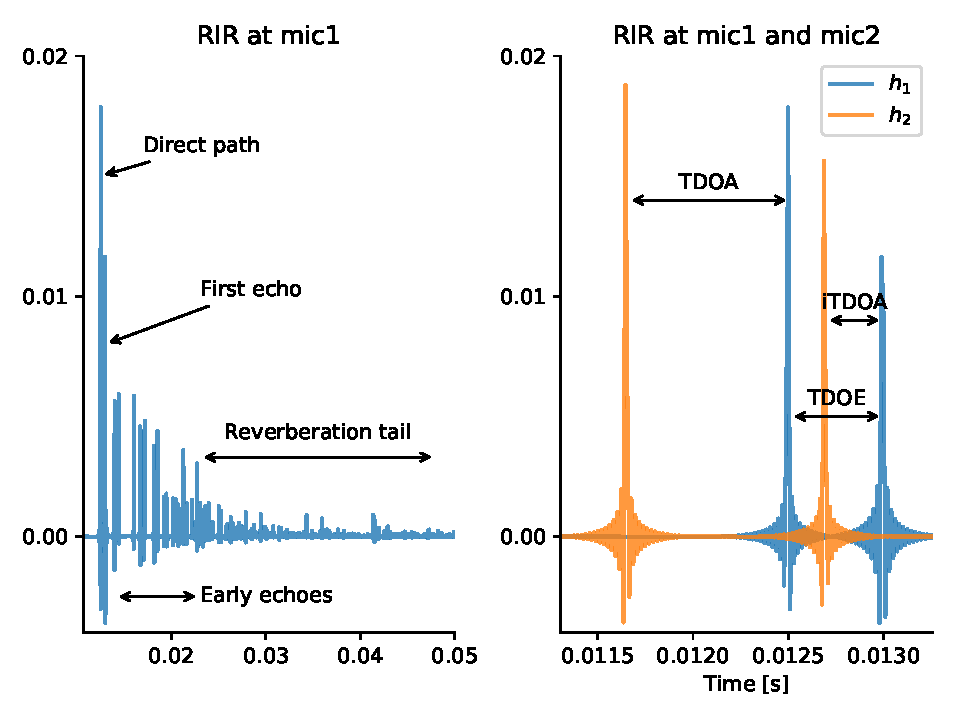
\includegraphics[trim={0 0 0 0},clip,width=\linewidth]{mirage/rirs.pdf}
    \end{sidecaption}
\end{figure}

\mynewline
Following the 2D-\SSL/ scheme described in \cref{subsec:mirage:2D-SSL} and given the virtual microphone-array geometry (which depends on the relative position of microphones to the surface),
$V$ could in principle be used to estimate the 2D directional of arrival of the source.
In the~\cref{ch:lantern}, we introduced a learning-based method to estimate $V$ using audio features obtained from only two microphones.

\mynewline
As stated is section \ref{subsec:mirage:2D-SSL}, given a microphone pair, the peak of angular spectrum $\Psi_\text{PHAT}$ corresponds to the \ac{TDOA}.
Moreover, peaks corresponding to the early reflection are presents.
\cref{fig:mirage:noise_ang_spec} shows the $\Psi_\mathtt{CC}$'s and the $\Psi_\mathtt{PHAT}$'s angular spectra for synthetic data where the source signal is noise or speech for all the pairs of the HARU's circular microphone array.
The location of the quantities in $V$ are highlighted with vertical dotted lines.
Theoretically, when only the first reflection are considered ($K=1$), the position of the peaks in the angular spectra correspond to
$\tau_\mathtt{TDOA}$, $\tau_\mathtt{iTDOA}$, $\tau_\mathtt{TDOA} - \tau_{\mathtt{TDOE}, 1}$, and $\tau_\mathtt{TDOA} + \tau_{\mathtt{TDOE}, 2}$.
It is important to note that for speech signals, $\Psi_\text{PHAT}$ removes the auto-correlation part in order to promote a sharp peak at the position of the \ac{TDOA}.
Since acoustic echoes increase the auto-correlations of the signal in one microphones, the \ac{PHAT} transform tends to lower their contribution, so that their peaks are not distinguishable from spurious ones.
\begin{figure}
    \begin{fullwidth}
        \centering
        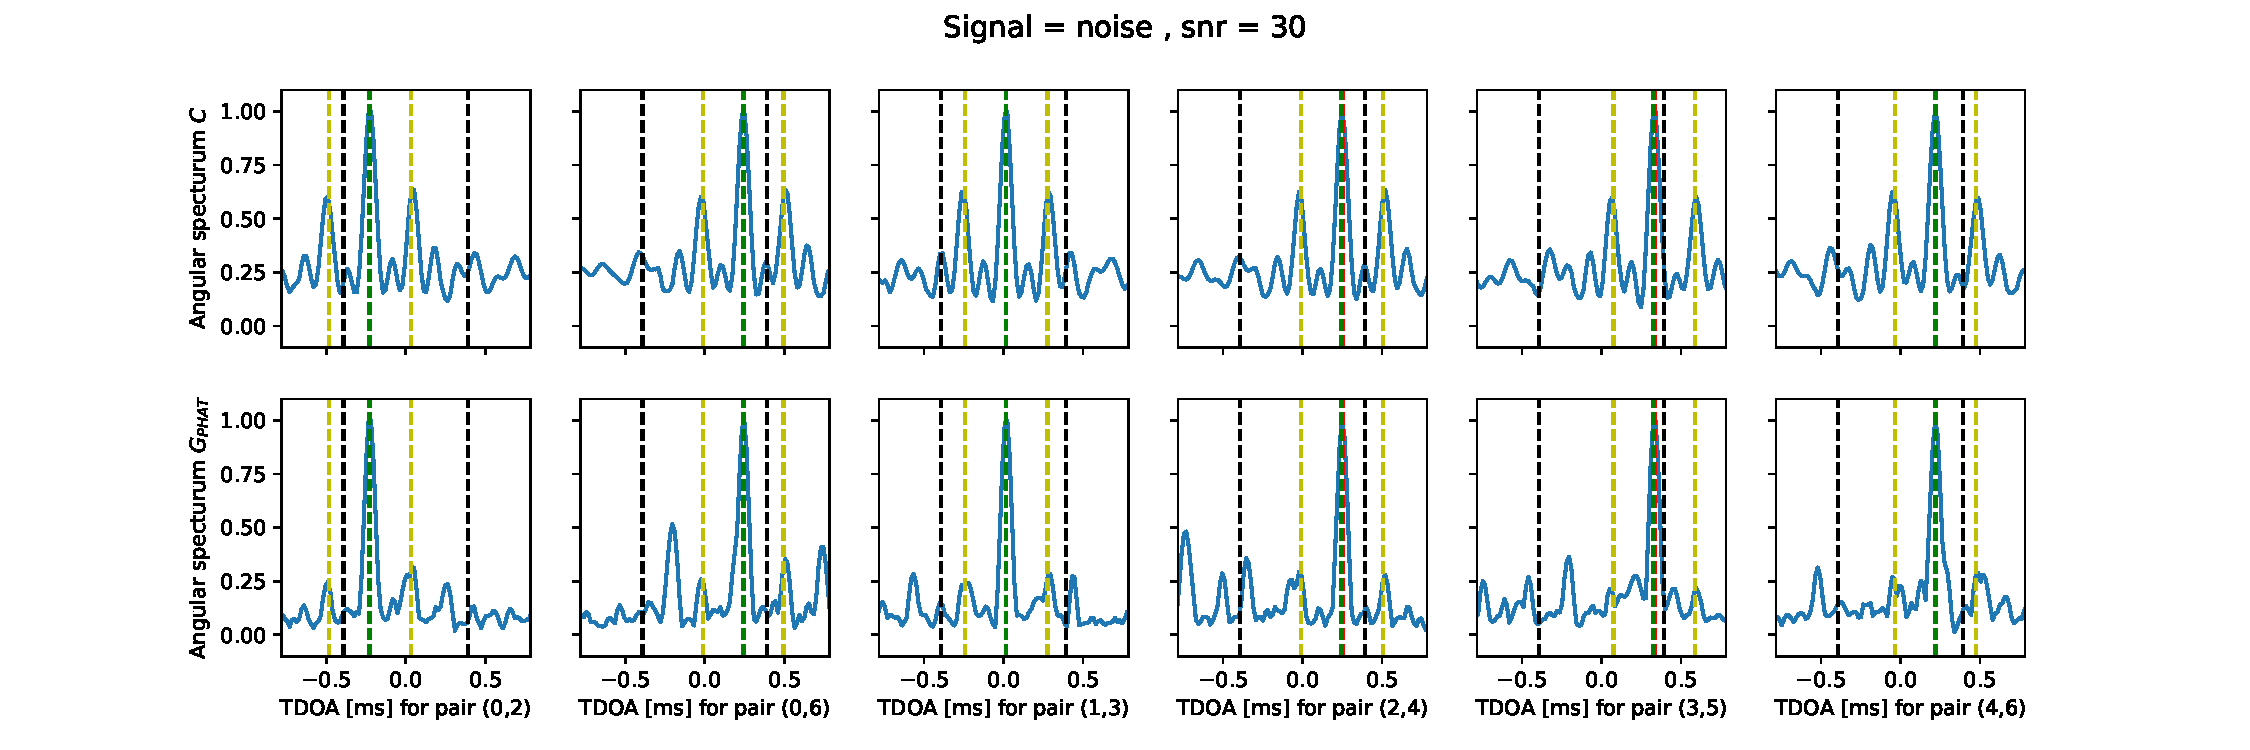
\includegraphics[trim={30mm 0 35mm 0},clip,width=\linewidth]{mirage/echo_hunting_broadband.pdf}
        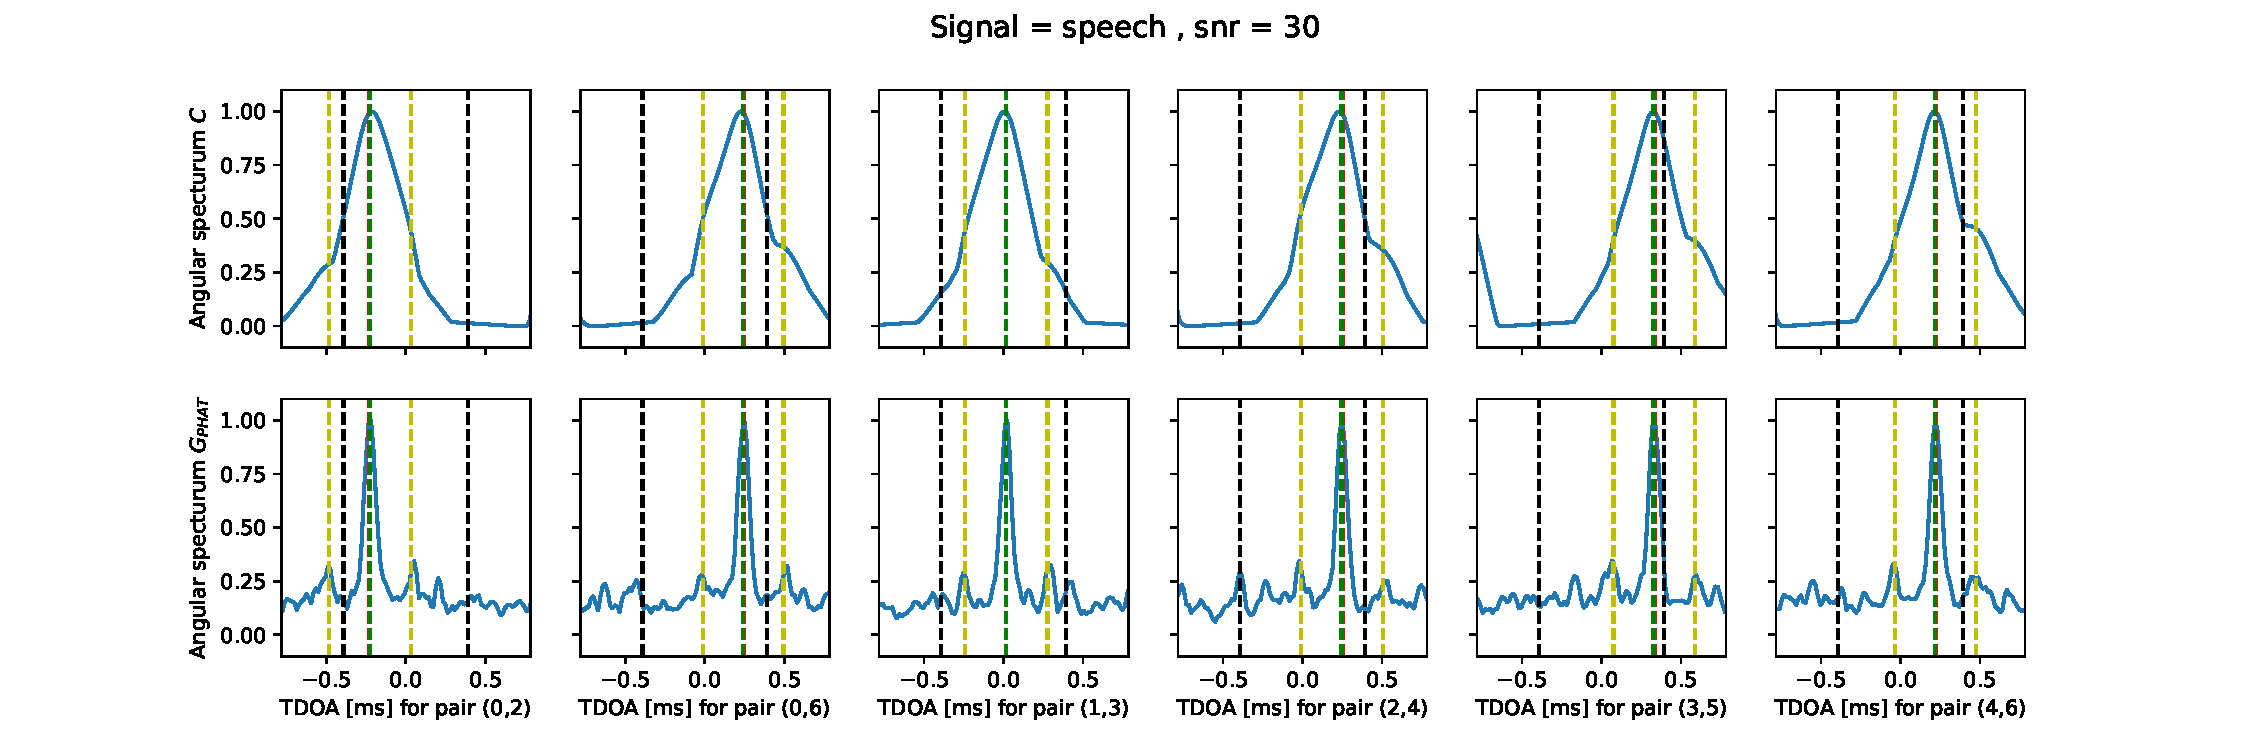
\includegraphics[trim={30mm 0 35mm 0},clip,width=\linewidth]{mirage/echo_hunting_speech.pdf}
        \caption{
            Angular Spectra $\Psi_\mathtt{CC}$ and $\Psi_\texttt{PHAT}$ for different pairs of microphone in the HARU array using synthetic \RIRs/ and \textit{white noise} (top) and \textit{speech} (botton) signal .
            Vertical lines mark the positions of  $\tau_\mathtt{TDOA}$ (red), $\tau_\mathtt{iTDOA}$ (green), $\tau_\mathtt{TDOA}-\tau_\mathtt{TDOE,1}$ (yellow) and $\tau_\mathtt{TDOA}+\tau_\mathtt{TDOE,2}$ (yellow) are marked with vertical lines.
            The black vertical lines correspond to the maximum TDOA given the pair distance, \textit{i.e.} corresponding to the AOA $ = \{0, 2\pi\}$}
        \label{fig:mirag:noise_ang_spec}
    \end{fullwidth}
\end{figure}


\section{Learning-based echo estimation}
We propose to use the learning-based approaches described in~\cref{ch:lantern} to estimated the quantities of interest $V$.
Our approach is to train a \ac{DNN} on a dataset simulating the considered close-surface scenario.
We model the problem as multi-target regression, with \acf{ILD} and \acf{IPD} as input features, and $V \in \mathbb{R}^3$ as output parameters.
As discussed in~\cref{subsec:processing:steering}, the \ac{ILD} and \ac{IPD} can be estimated from the \STFT/ of the microphone signals, such as,
\begin{equation} \label{eq:mirage:features}
\begin{cases}
\ild[k]  =& \tfrac{1}{T} \sum_{l=1}^T \log{\abs{\frac{\MIC_2[k,l]}{\MIC_1[k,l]}}} \\
\ipd[k]  =& \tfrac{1}{T} \sum_{l=1}^T \frac{\MIC_2k,l]/ \abs{\MIC_2[k,l]}}{ \MIC_2k,l] / \abs{\MIC_1[k,l]}}\\
\end{cases}
\end{equation}
More precisely, the input of the network is $\klist{ \ild, \kRe\set{\ipd}, \kIm\set{\ipd}}$, where $\kRe\set{\cdot}$ and $\kIm\set{\cdot}$ denote real and imaginary part operators, respectively.
Note that for the \ac{IPD}, the frequency $k=0$ is discarded because it is constant for every observation.

% \mynewline
% In general, the mapping between $V$ and the proposed feature is not unique.
% In particular, this happen when $\tau_2^1 = \tau_1^1$.
% In order to avoid this, we preventively pruned all the entries with $| \tau_2^1 - \tau_1^1 | < 10^{-6}$ from the dataset.

\subsection{TDOA estimation with simple neural networks}
As first investigation, we used the simple \ac{MLP} architecture consisting described in~\cref{sec:lantern:mlp}.
For the paper~\citeonly{di2019mirage} we used the following implementation:
a $D$-dimensional input layer, a 3-dimensional output layer, and 3 fully connected hidden layers with respective input sizes $500$, $300$ and $50$.
Rectified linear unit (ReLU) activation functions are used except at the output layer, and each hidden layer has a dropout probability $p_\text{do} = 0.3$.

\mynewline
We use the mean square error loss function for training and the Adam optimizer \citeonly{kingma2014adam}.
The \acf{nRMSE}  is taken as validation metric\sidenote{
    The ac{nRMSE} takes values between $0$ (perfect fit) and $\infty$ (bad fit).
    If it is equal to $1$, then the prediction is no better than a constant.
}.
The network is manually tuned on a validation set to find the best combination of number of hidden layers, their sizes and $p_\text{do}$.

\mynewline
Once time delay estimates $\hat{V}$ are returned by the \ac{MLP}, they are converted to \textit{synthetic local angular spectra} and passed to $\Psi_\text{SRP}$ (See~  \cref{subsec:mirage:2D-SSL})
together with the relative positions of true and image microphones which are assumed known.
The synthetic local angular spectra consist of Gaussian functions centered at $\hat{V}$ and with variances equal to the prediction errors made by the \ac{MLP} on the validation set.

\subsection{Robust TDOA estimation with convolutional neural network}

\section{Experimental Results}\label{sec:mirage:exp}

\subsection{2-channel scenario}
To the best of the authors' knowledge, no reference implementation of algorithms for 2D-SSL using only 2 microphones is available to date.
To check the validity of \ac{TDOA}s estimation, our approach is compared to \ac{GCC-PHAT} using only the true microphones (see Sec. \cref{subsec:mirage:1D-SSL}).

\mynewline
The \ac{DNN} model is trained and validated on many random, shoe-box room configurations generated by the software presented in \citeonly{schimmel2009fast}.
This software implements both the image-method for simulating reflections and a ray-tracing algorithm for diffusion.
Room widths are uniformly drawn at random in $[3, 9]$~m, heights in $[2, 4]$~m.
Random source/microphones positions and absorption coefficients for the 6 surfaces are used,
respecting the close-surface scenario. In particular, the microphones are at most $30$ cm from the close-surface,
placed $10$ cm from each other, the absorption coefficients of the other walls are
uniformly sampled in $(0.5, 1)$ and the one of the close-surface is in $(0, 0.5)$.
The same realistic diffusion profile \citeonly{gaultier2017vast} is used for all surfaces.
Around $90,000$ audio scenes are generated this way, yielding reverberation time \RT{} between $20$~ms and $250$~ms.

\mynewline
For both training and validation, the \acp{RIR} are convolved with 1~second of white-noise (wn) with no additional noise.
All signals and RIRs are sampled at $\SI{16}{kHz}$.
The \STFT/ is performed on 1024 point with 50\% overlap.
Finally, the features are computed as in~\eqref{eq:mirage:features} yielding a vector of size $D = 1534$ for each observation.
While we validate the MLP on a portion of the dataset in a \textit{holdout} fashion, the test is conducted on 200 new \acp{RIR} convolved with both wn and speech (sp) utterances.
This set is generated similarly to the training and validation sets. Moreover the recordings are perturbed by external white noise at 10 dB SNR (wn+n, sp+n).
The speech signals are normalized speech utterances of various lengths (from $1$ s to $6$ s), randomly selected from the TIMIT corpus.
A free and open-source Matlab implementation of \ac{SRP-PHAT}\sidenote{\href{http://bass-db.gforge.inria.fr/bss_locate/}{MBSSLocate\ExternalLink}} is used to aggregate local angular spectra obtained from the \ac{DNN}'s output.
The same toolbox is used for the implementation of \ac{SRP-PHAT} with \ac{GCC-PHAT}.
For the latter method only real pairs are used.
A sphere sampling with $\ang{0.5}$ resolution and coordinates $\theta \in [-179, 180]$ and $\phi \in [0, 90]$ is used for the \c{DOA} search.

\begin{table}[ht!]
    \begin{sidecaption}[Echo estimation with MIRAGE results]{%
        Normalize root mean squared error for TDOA estimation and mean angular error in ${}^\circ$ (with accuracies ($\%$))
        for AOA estimation with $\ang{10}$ and $\ang{20}$ angular tolerance.
    }[tab:mirage:tdoas-aoa]
    \centering
    \footnotesize
    %\scriptsize
    \begin{tabular}{cl|ccc|cc}
    \toprule
                &         &          & nRMSE        &                   &\multicolumn{2}{c}{ACCURACY}  \\
                & Input   &    \scriptsize{TDOA}  	&   \scriptsize{iTDOA} 		 &     \scriptsize{TDOE} 		 & $\theta<\ang{10}$ &  $\theta<\ang{20}$ \\
    \midrule
    MIRAGE      &   wn    & 0.18    & 0.28  & 0.25 	& 4.10 (77)	& 5.97 (97) \\
    MIRAGE      &   wn+n  & 0.68    & 0.69  & 0.89 	& 5.00 (26)	& 9.89 (54) \\
    MIRAGE      &   sp    & 0.31    & 0.34  & 0.56  & 4.83 (63)	& 7.26 (82) \\
    MIRAGE      &   sp+n  & 0.99    & 0.98  & 1.48 	& 4.60 (16)	& 9.88 (35) \\
    GCC-PHAT    &   wn    & 0.21    & -     & -		& 4.22 (81) & 6.19 (97) \\
    GCC-PHAT    &   wn+n  & 0.68    & -     & -		& 4.03 (65) & 5.34 (83) \\
    GCC-PHAT    &   sp 	  & 0.32    & -     & -		& 4.08 (82) & 5.34 (97) \\
    GCC-PHAT    &   sp+n  & 1.38    & -     & -		& 4.70 (19) & 8.38 (32) \\
    \bottomrule
    \end{tabular}
    \end{sidecaption}
\end{table}

\begin{table}[ht]
\begin{sidecaption}[DoA estimation]{%
    Mean angular error in degree (with accuracies ($\%$)) for 2D SSL (azimuth and elevation)
    with $\ang{10}$ and $\ang{20}$ tolerance.}[tab:mirage:doa]
    \footnotesize
    \centering
    \begin{tabular}{cl|cc|cc}
    \toprule
    \textbf{DoA}    &            &  \multicolumn{2}{c|}{ACCURACY}    &   \multicolumn{2}{c}{ACCURACY} \\
                    &            &  \multicolumn{2}{c|}{$<\ang{10}$} &   \multicolumn{2}{c}{$<\ang{20}$} \\
                    &    Input   &  $\theta$ &  $\phi$ &  $\theta$ &  $\phi$ \\
    \midrule
    MIRAGE &  wn    &   4.5 (59) &  3.9 (71) &   6.8 (79) &   5.9 (88) \\
    MIRAGE &  wn+n  &   4.4 (18) &  5.5 (26) &   9.4 (35) &  11.1 (66) \\
    MIRAGE &  sp    &   4.6 (45) &  4.8 (59) &   8.1 (71) &   7.2 (83) \\
    MIRAGE &  sp+n  &   5.2 (17) &  5.9 (12) &  10.7 (38) &  12.3 (43) \\
    \bottomrule
    \end{tabular}
\end{sidecaption}
\end{table}

\ac{TDOA} estimation errors using the proposed approach and \ac{GCC-PHAT} are presented in Table~\cref{tab:mirage:tdoas-aoa}.
Training a \ac{DNN} to estimate \acp{TDOA} brings similar performances as \ac{GCC-PHAT} in terms of \ac{nRMSE}.
Estimation of \acp{iTDOA} and \ac{TDOE} seems to be a harder task for the simple \ac{DNN} we used.
Nevertheless, our results confirm the possibility of retrieving early echoes from only two-microphone recordings.
When some external noise is added, performance of both methods severely degrades.
This is a well-know and expected behavior for \ac{GCC-PHAT}.
It suggests that noise should be considered in the training phase of \MIRAGE/.
When we compare the performance in terms of \ac{AOA}, the two methods yield the same accuracy within a $\ang{20}$ threshold, as can be see in Table~\cref{tab:mirage:tdoas-aoa}.
When a smaller tolerance is considered, GCC-PHAT outdoes the proposed approach in accuracy, with comparable errors.
This behavior is due to two aspects: first, the synthetic angular spectrum is might be a too simple model; second, since \ac{nRMSE} was chosen as validation metrics, accuracy is not directly optimized.
Again, when adding noise, performance decreases.

\mynewline
In Table~\cref{tab:mirage:doa} the performance of the full 2D-SSL pipeline is showed.
Within a tolerance of $\ang{20}$, the \MIRAGE/ model allows estimation of both azimuth and elevation of the target source.
However since in our data the 2 microphones were free to move, the inclinations of the true and image pairs are rarely flat.
While this helps elevation estimation, it reduces the accuracy of predicting the right azimuth.
While external noise is again decreasing the accuracy dramatically,
it is interesting to notice that our \ac{DNN} model trained and validated with white noise sources somewhat generalizes to speech sources.

\mynewline
In this paper we demonstrated how a simple echo model could allow 2D SSL with only two microphones, using simulated data.
Future research will focus on extending this proof-of-concept to real data.
The problem of echo-delay estimation proved to be very challenging, and extensions of the proposed learning scheme will be developed to obtain more reliable estimations of angular spectra.
Extensions of the method to better handle various types of noise and emitted signals will also be sought.
Finally, applications of the MIRAGE framework to larger microphone arrays, higher order echoes and a variety of tasks beyond SSL will be explored.


\subsection{Multi-channel scenario}



\section{Conclusion}
In this work, we demonstrated how a simple echo model could boost performance in 2D \ac{SSL} in strongly echoic scenarios, that is, when microphones are placed close to a reflector.
Preliminary results on synthetic data for stereophonic recordings prove the effectiveness of the approach and were presented in a international conference paper.
However, results obtained on real data reveal that the task is still very challenging, both for the proposed method and the baseline.
New data collection must be considered in order to fully assess the proposed approach.
In general, the results are encouraging and suggest that modeling echoes can significantly reduce the number of gross \ac{SSL} errors that are observed using baseline methods in strongly echoic environment.
Further investigation is needed to strengthen these results and further improve the robustness of the learned mapping.
In particular, methods that handle missing frequencies at the \ac{DNN}'s input will be considered.

